
\subsection{Analysis of Critical Time}


When the simplified and the extended models of the IEEE benchmark are compared for the estimation of the critical time in Figure \ref{fig:res_tcr}, it is noticed a higher deviation in the low range of RoCoF. This because in this range of RoCoF the critical time is long enough to allow the governor response activation of the respective synchronous machines representation. Therefore it can be stated that the simplifications made in the model have a greater influence on the results for low values of penetration of IBG and low power imbalances; in this sense, the simplifications become less significant as the RoCoF increases in such a manner that the activated synchronous reserve is not relevant in frequency support. In the range of RoCoF higher than 2 Hz/s the critical time trend for the European grid-scale and the simplified IEEE model get closer each to other as RoCoF increases.

\begin{figure}[h]
	\centering
	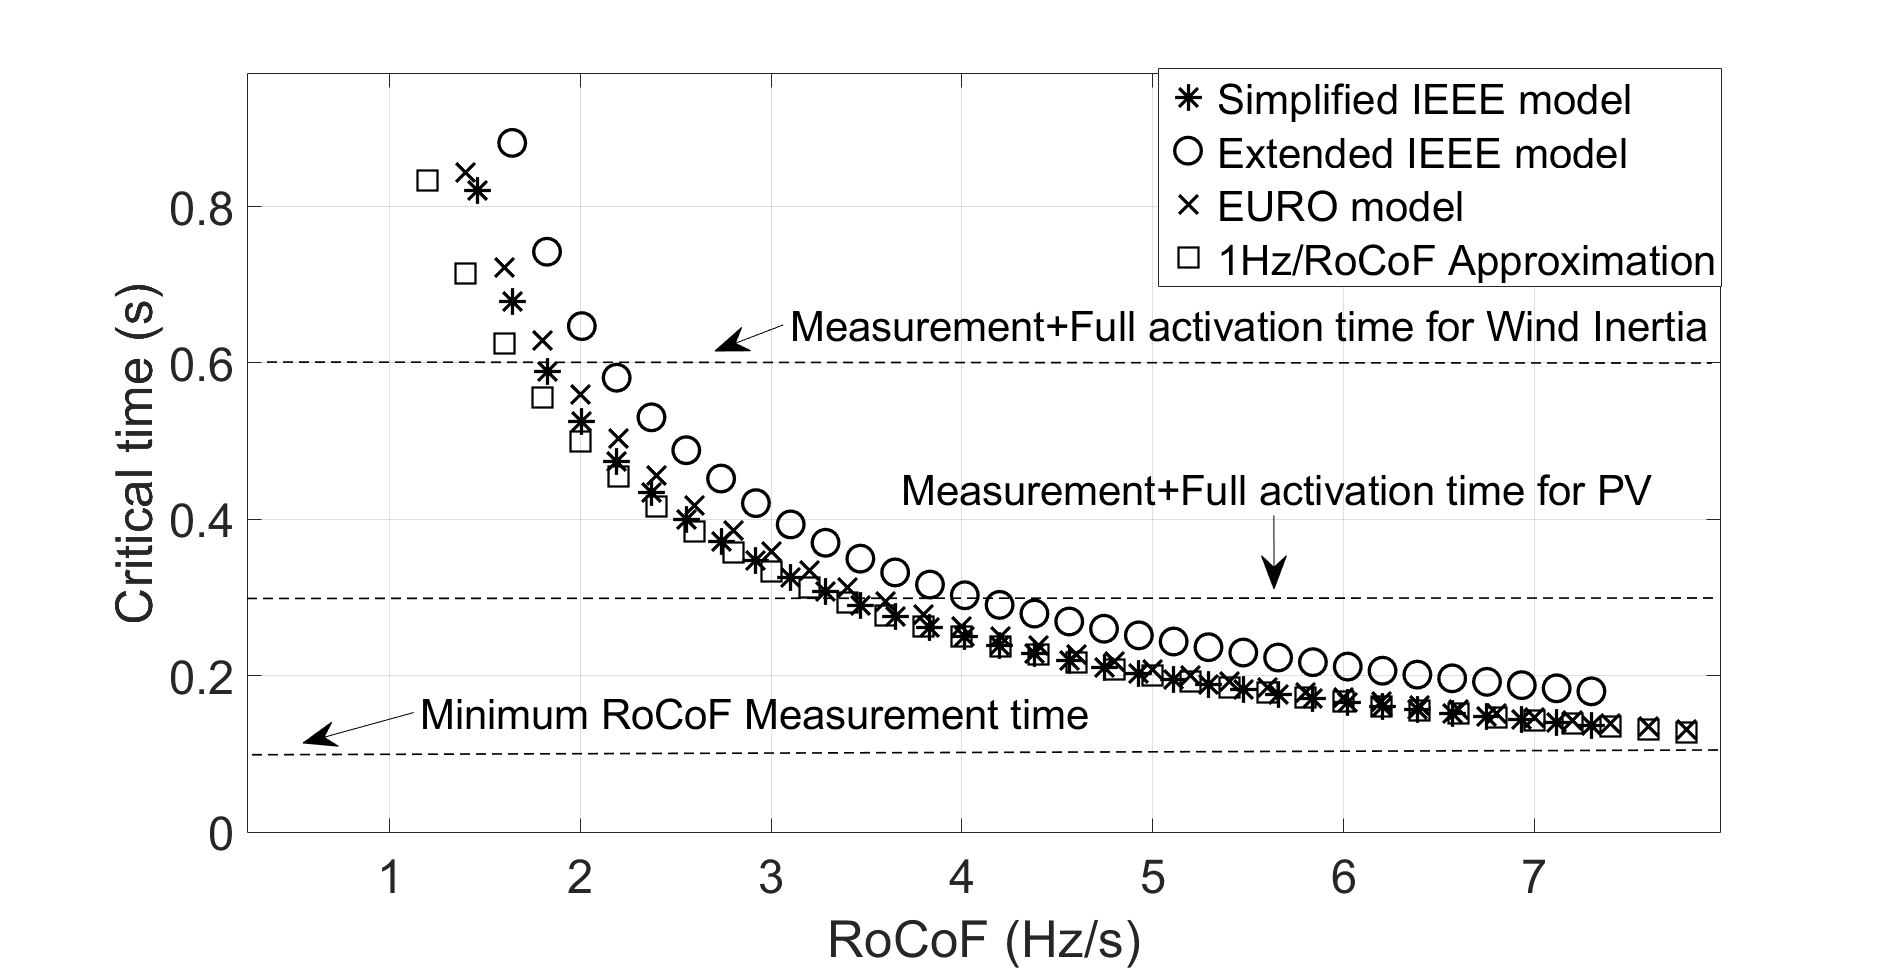
\includegraphics[width=0.6\textwidth]{/result/tcr80}
	\caption{Results for critical time in all simulated models with a penetration of IBG of 80\% .}
	\label{fig:res_tcr}
\end{figure}


Therefore under high RoCoF conditions in any of the models, the primary reserve does not significantly counteract the frequency drop \cite{dena2014}. Figure \ref{fig:res_tcr} demonstrates that primary reserve can be neglected for determining the critical time when the combination of IBG and load imbalances would lead to high values of RoCoF; as it increases, the approximation of critical time as 1 Hz/RoCoF narrows the difference with the results obtained from simulations \cite{miller2017technology}. Nevertheless, such simplification applies to the simplified IEEE model and the European-scale grid model. Hence, the influence of all the dynamics and machine components, such as the generator exciter and damping windings, seems to improve the critical time. The damping torque was not considered in Equation \eqref{eq:swing} for the simplified IEEE model; the inclusion of such may lead to more accurate results when compared with the extended model.
\begin{table}[h]
	\caption{\label{tb:crtime}: Critical time for European-scale case given in seconds.}
	\centering
	%% \tablesize{} %% You can specify the fontsize here, e.g., \tablesize{\footnotesize}. If commented out \small will be used.
	\begin{tabular}{*9c}
		\toprule
		\textbf{IBG share (\%)}    & \multicolumn{8}{c}{\textbf{Load Imbalance (\%)}} \\
		\midrule
		{} & 3&    4&    5&    6&    7&    8&    9    &10 \\
		\midrule
		20&    -    &    -    &    6.081&    4.517&    3.629&    3.050&    2.638&    2.316\\
		40&    -    &    6.226&    4.169&    3.215&    2.628&    2.222&    1.934&    1.705\\
		60&7.142 &    3.639&    2.623&    2.062&    1.698&    1.451&    1.263&    1.122\\
		80&    2.753&    1.744&    1.277&    1.018&    0.843&    0.722&    0.628&    0.559\\
		
		95&    0.697&    0.436&    0.322&    0.254&    0.211&    0.179&    0.157&    0.140\\
		\bottomrule
	\end{tabular}
\end{table}


Because the characteristics of the  European interconnected scenario provided by ENTSOE were assumed to be the same as the resulting islands after a severe event; the results for the large scale model can be understood as the behavior of the whole European system with bigger perturbations. The reference scenario assumes a power imbalance of 3 GW, which corresponds to a 2\% of the 150 GW load \cite{ENTSOE.2016}. If in the future a bigger reference scenario is utilized, then the synchronous response would not be enough to balance the system before load shedding occurs. Table \ref{tb:crtime} exhibits the required time when the power imbalance is increased by up to 10\% for different IBG penetration.



\subsection{Analysis of Synthetic Inertia and Fast Power Reserve}




\subsubsection{Effect Synthetic Inertia on Frequency}
\label{sec:res_si}
In this section, the results of the implementation of synthetic inertia in the simplified IEEE model and the European model are presented. The frequency nadir for such systems without any additional power support apart from synchronous response are illustrated in Figures \ref{fig:res_nadirieee_simp} and \ref{fig:res_nadireuro}.\\

\begin{figure}[h]
	\centering
	\begin{subfigure}[h]{0.49\textwidth}
		\centering
		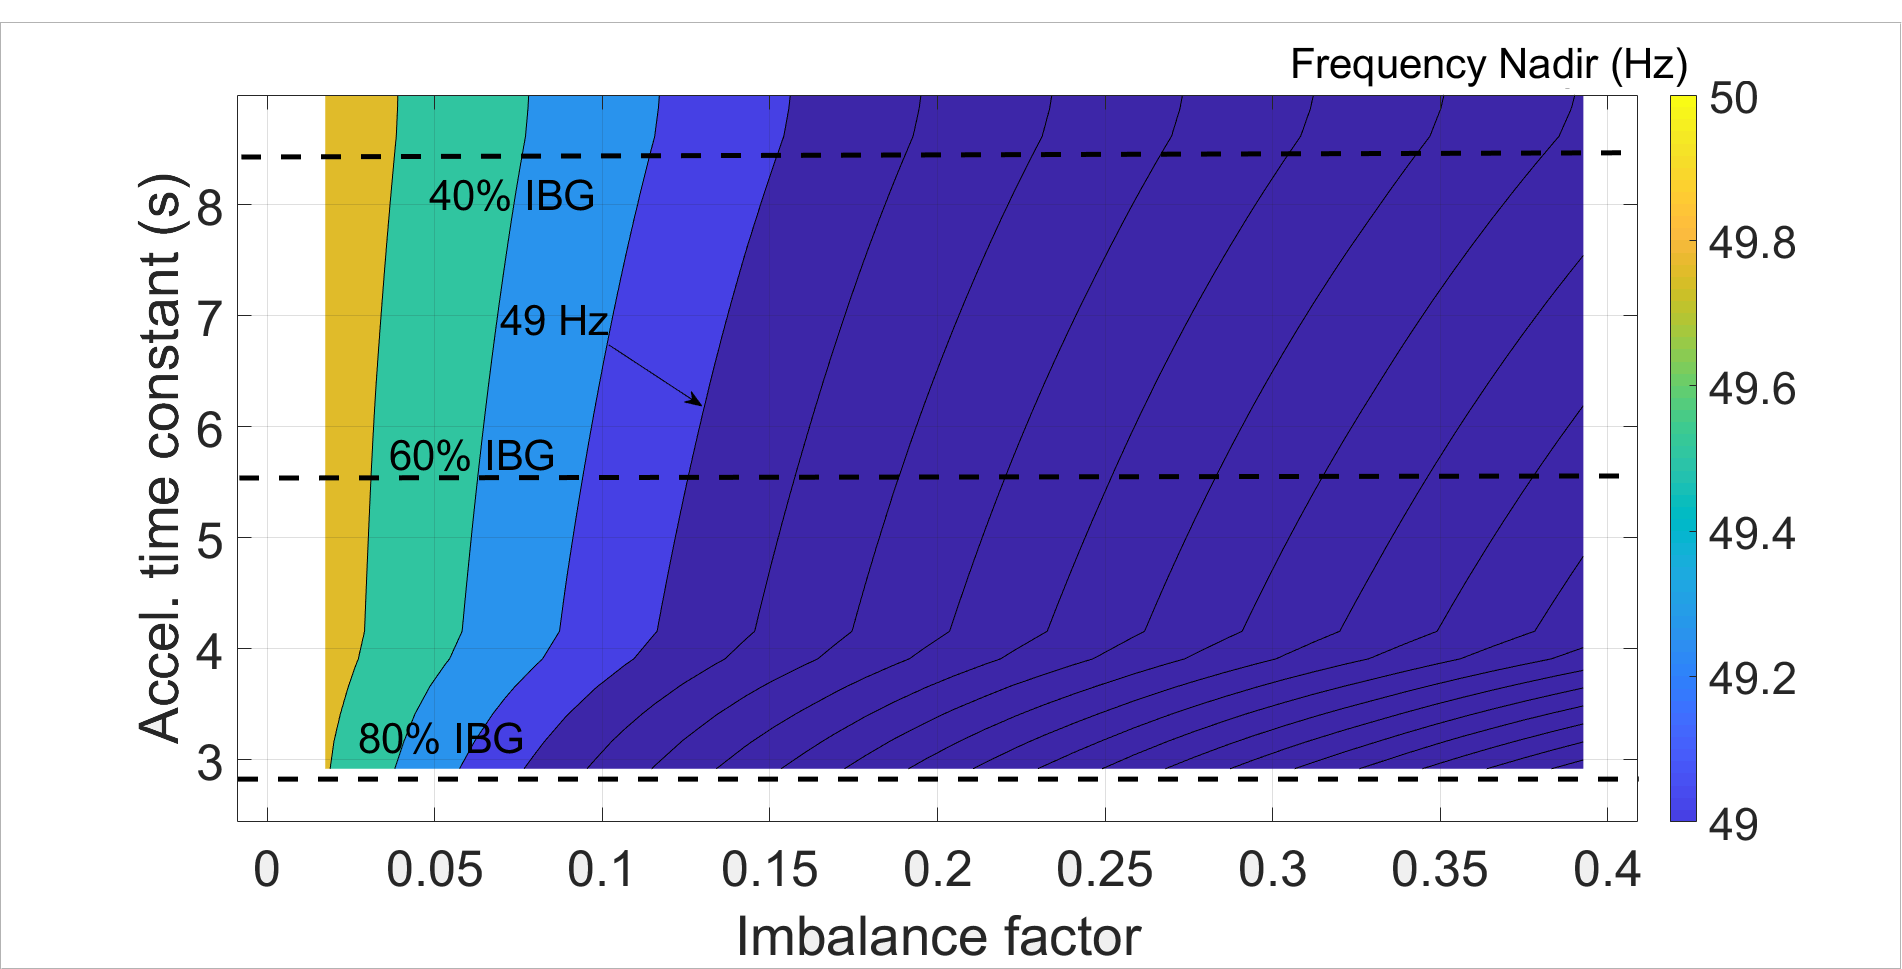
\includegraphics[width=\textwidth]{result/base}
		\caption{Simplified IEEE model}
		\label{fig:res_nadirieee_simp}
	\end{subfigure}
	\hfill
	\begin{subfigure}[h]{0.49\textwidth}
		\centering
		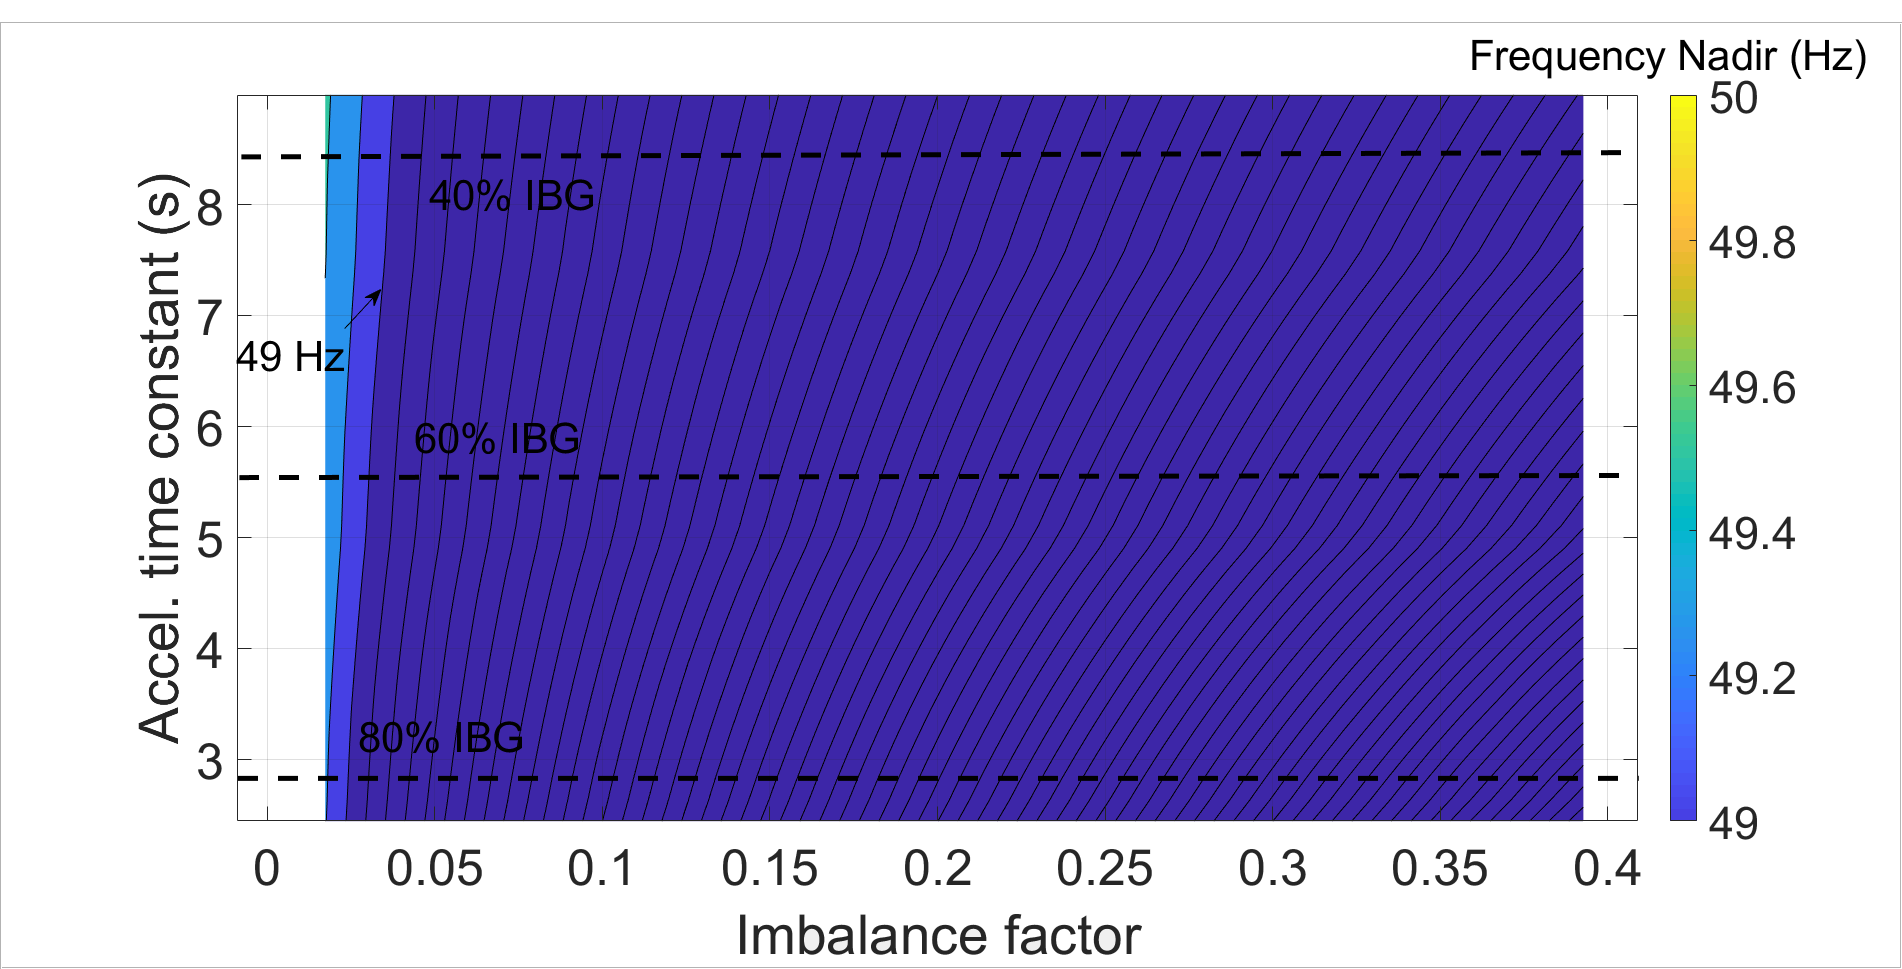
\includegraphics[width=\textwidth]{result/base_euro}
		\caption{European-scale model}
		\label{fig:res_nadireuro}
	\end{subfigure}
	
	
	\caption{Frequency nadir with no support from IBG. (\textbf{a}) The frequency nadir of the simplified IEEE model. For the time acceleration constant corresponding to the 80\% of the IBG, the frequency nadir reaches values lower than 49 Hz with power imbalances starting at $ \sim 7\% $. In (\textbf{b}) the frequency nadir of the European-scale grid is illustrated. At 80\% of IBG the frequency nadir reaches 48.73 Hz with only $\sim 3\% $ of imbalance.}
\end{figure}

In any of the cases, UFLS is not avoided for all combination of imbalances and acceleration constants with the application of synthetic inertia. It can also be observed in Figure \ref{fig:res_nadirieee_si} that values of frequency nadir under 49 Hz are reached for imbalances bigger than 14\% combined with shares of IBG above 80\% in the simplified representation of the IEEE model. Nevertheless, enhanced performance is observed in the simplified IEEE model. The reason behind this is the faster response of the synchronous share present in the system, which jointly performs with the synthetic inertia to improve overall frequency response performance. On the other hand, the frequency nadir of the European scale model, depicted in Figure \ref{fig:res_nadireuro_si} at 80\% of IBG, reaches 48.89 Hz with an imbalance of 3\%. This demonstrates that synthetic inertia is not enough by itself for withstanding severe imbalances under high penetration of inverter-based generation.\\
\begin{figure}[h]
	\centering
	\begin{subfigure}[h]{0.49\textwidth}
		\centering
		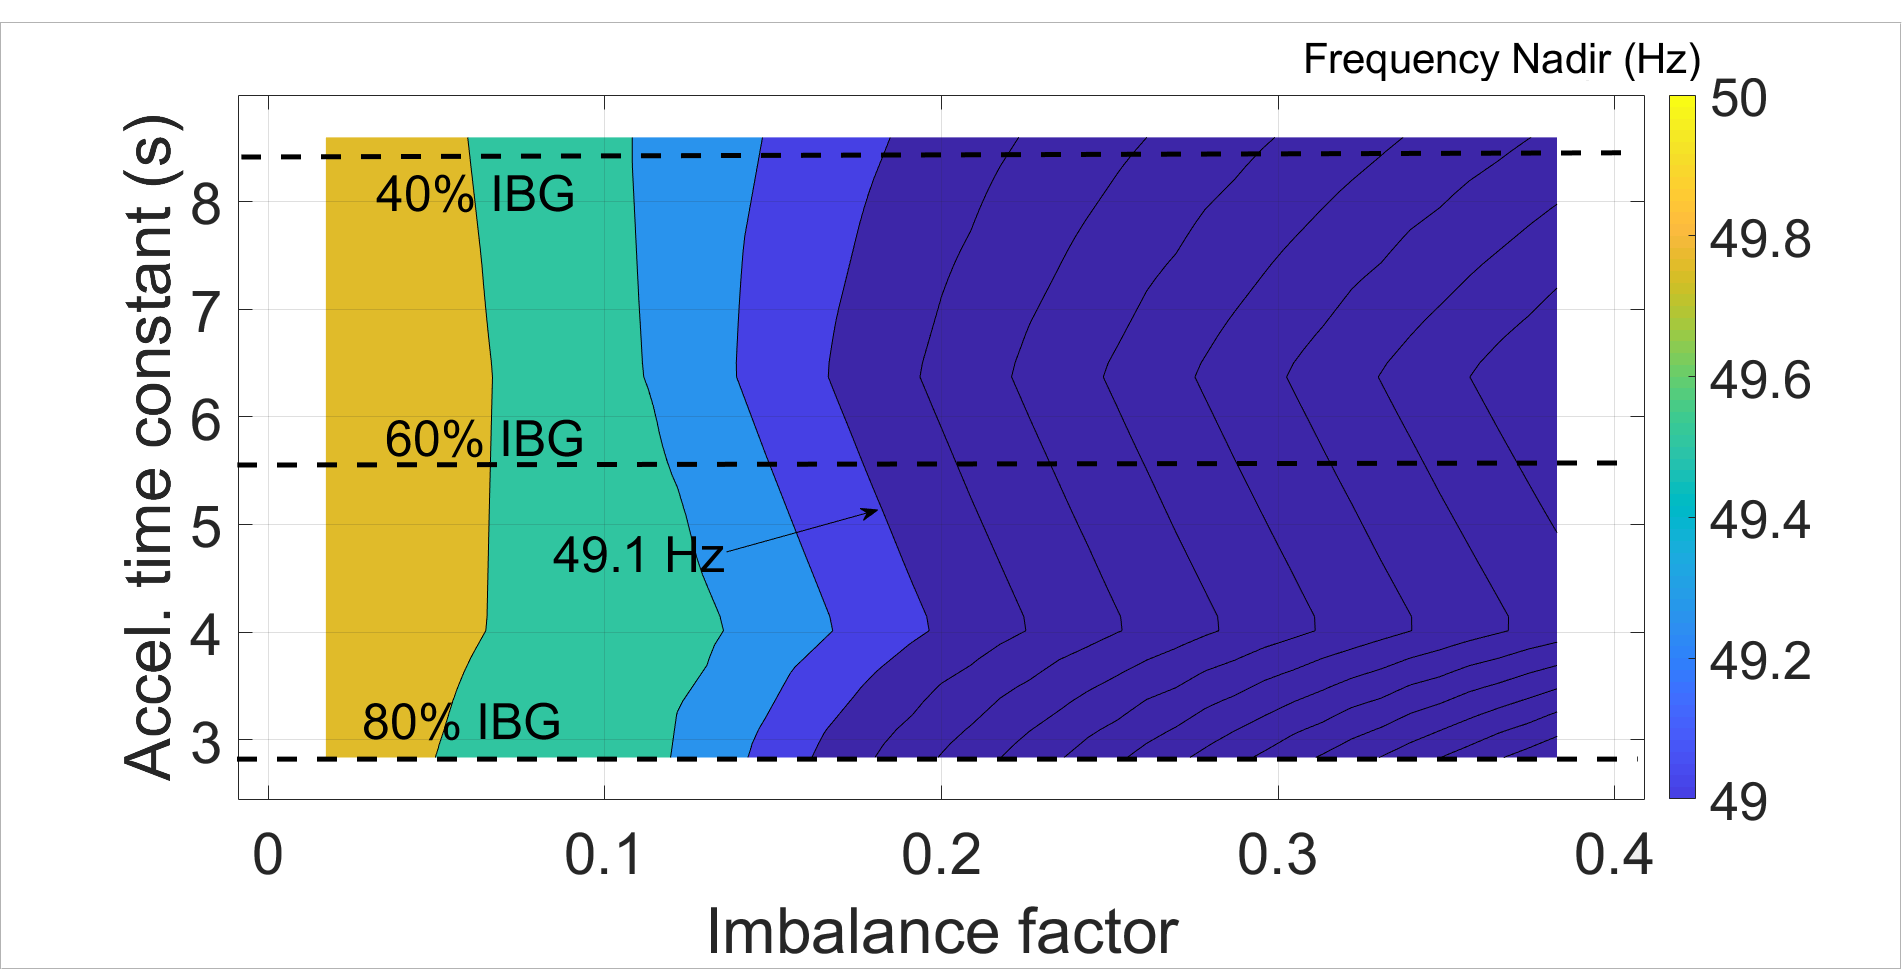
\includegraphics[width=\textwidth]{result/SI40}
		\caption{Simplified IEEE model.}
		\label{fig:res_nadirieee_si}
	\end{subfigure}
	\hfill
	\begin{subfigure}[h]{0.49\textwidth}
		\centering
		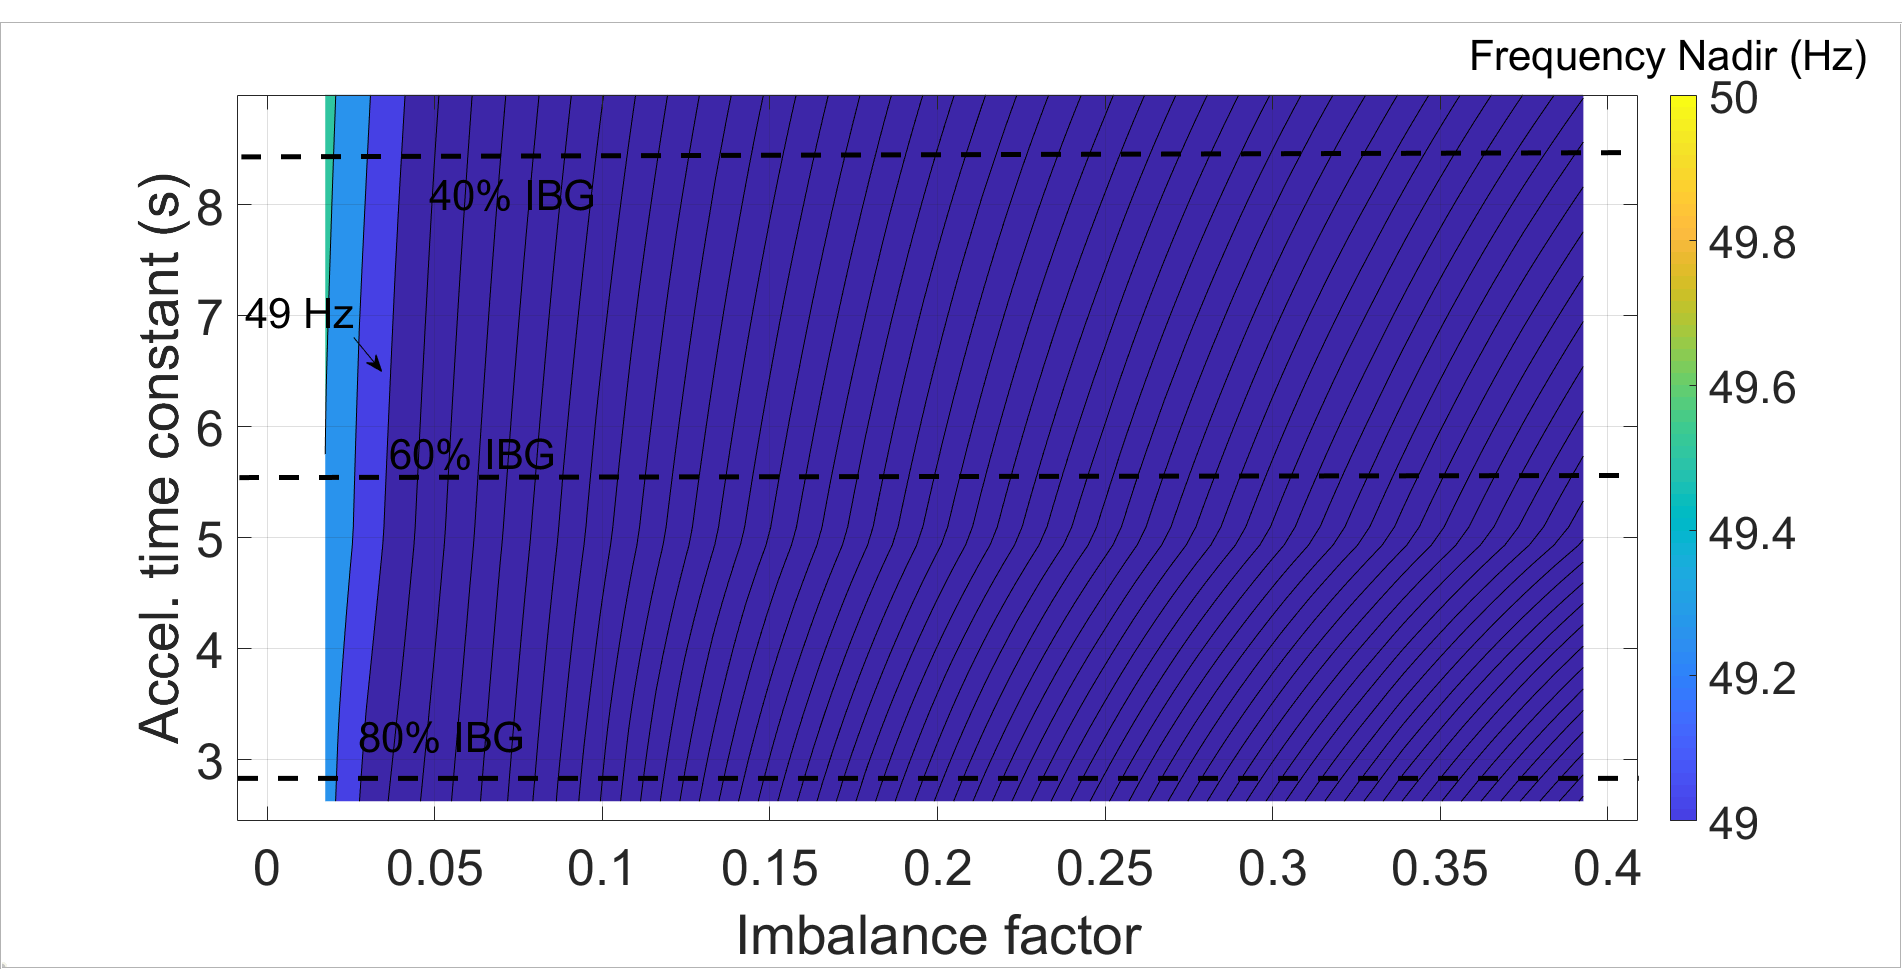
\includegraphics[width=\textwidth]{result/SI80Euro}
		\caption{European-scale model.}
		\label{fig:res_nadireuro_si}
	\end{subfigure}
	
	
	\caption{(\textbf{a}) Shows the frequency nadir once synthetic inertia has been applied to the 40\% of the IBG in the simplified IEEE model. (\textbf{b}) Frequency nadir of the large scale model with the same share of contribution from synthetic inertia.}
\end{figure}


Figure \ref{fig:res_ieee_fr10imb} and \ref{fig:res_ieee_fr15imb} indicate the frequency response obtained of the system with an non-synchronous generation of 80\% for different load imbalances.  In Figure \ref{fig:res_ieee_fr10imb} can be observed how the frequency drops below 49 Hz with a 10\% of imbalance when no IBFPR or synthetic inertia is used as a frequency support strategy. In the same figure, the frequency responses for different levels of synthetic inertia is presented. It is noticed the improvement in the response with the implementation of synthetic inertia. UFLS is avoided for every share of synthetic inertia, assuming that primary reserve takes place after synthetic inertia. As the imbalance increases, the effectiveness of the synthetic inertia decreases. 

\begin{figure}[h]
	\centering
	\begin{subfigure}[h]{0.49\textwidth}
		\centering
		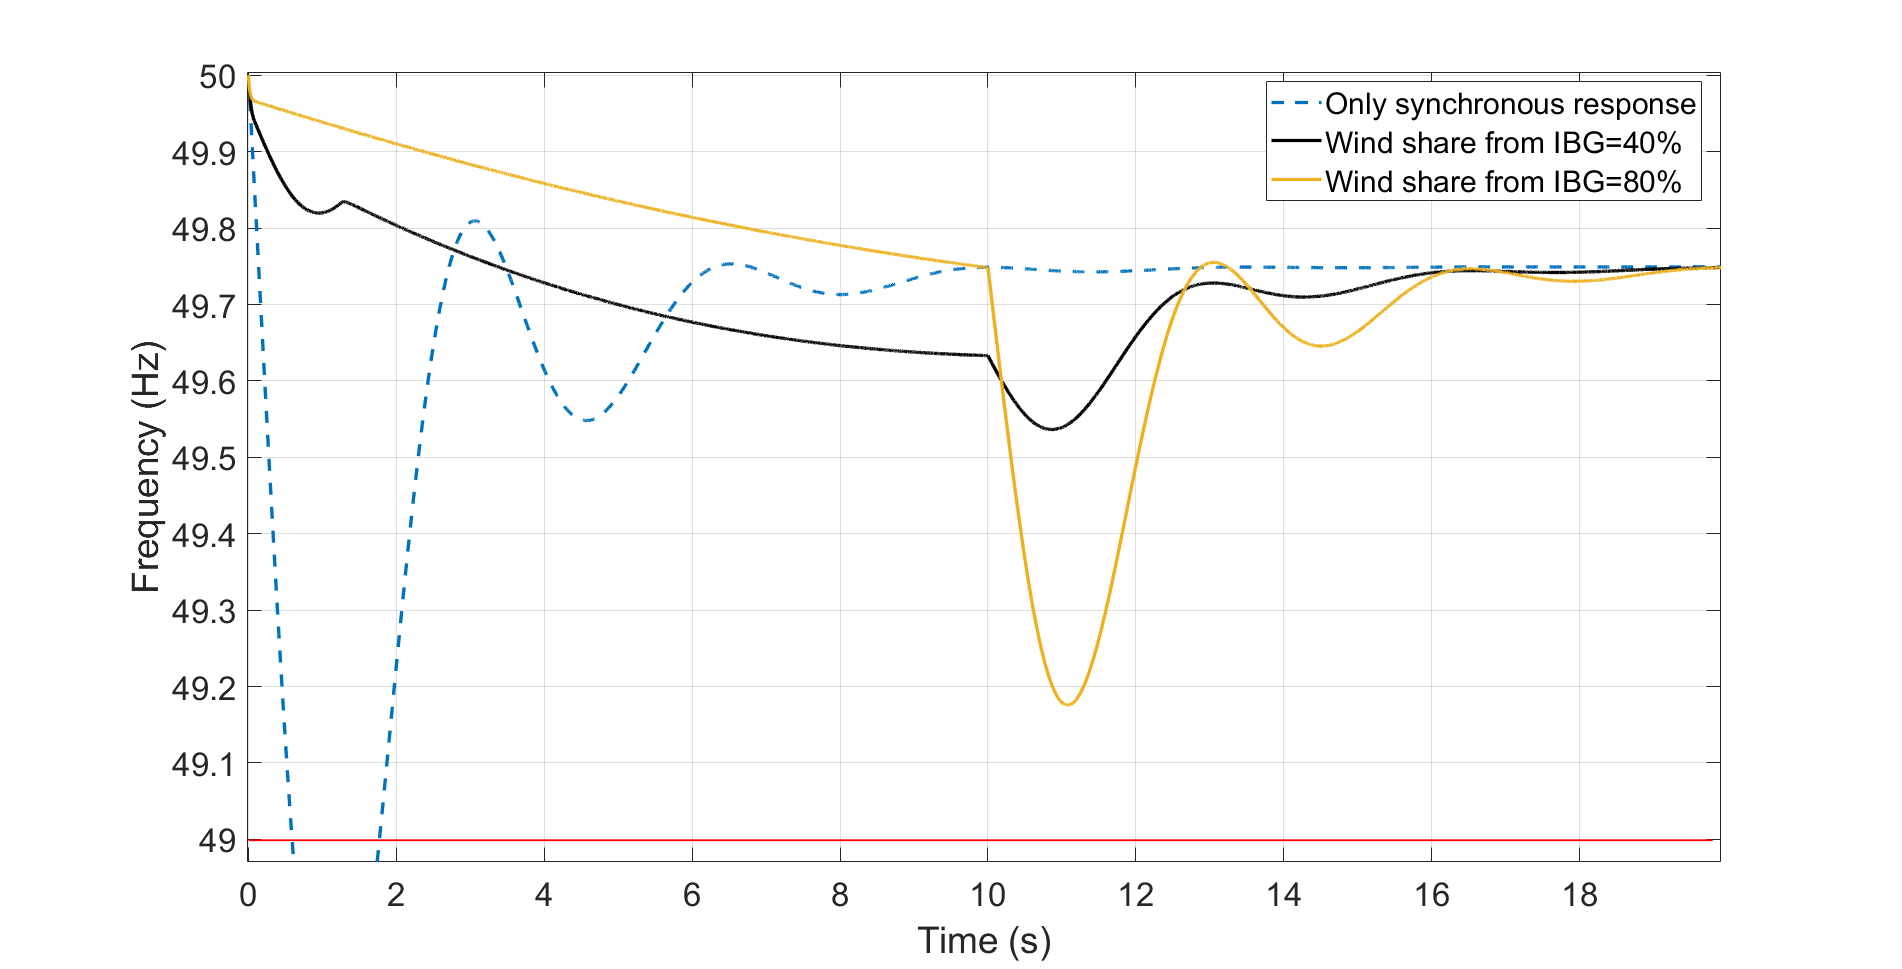
\includegraphics[width=\textwidth]{result/SI10imb}
		\caption{Simplified IEEE model with 10\% imbalance}
		\label{fig:res_ieee_fr10imb}
	\end{subfigure}
	\hfill
	\begin{subfigure}[h]{0.49\textwidth}
		\centering
		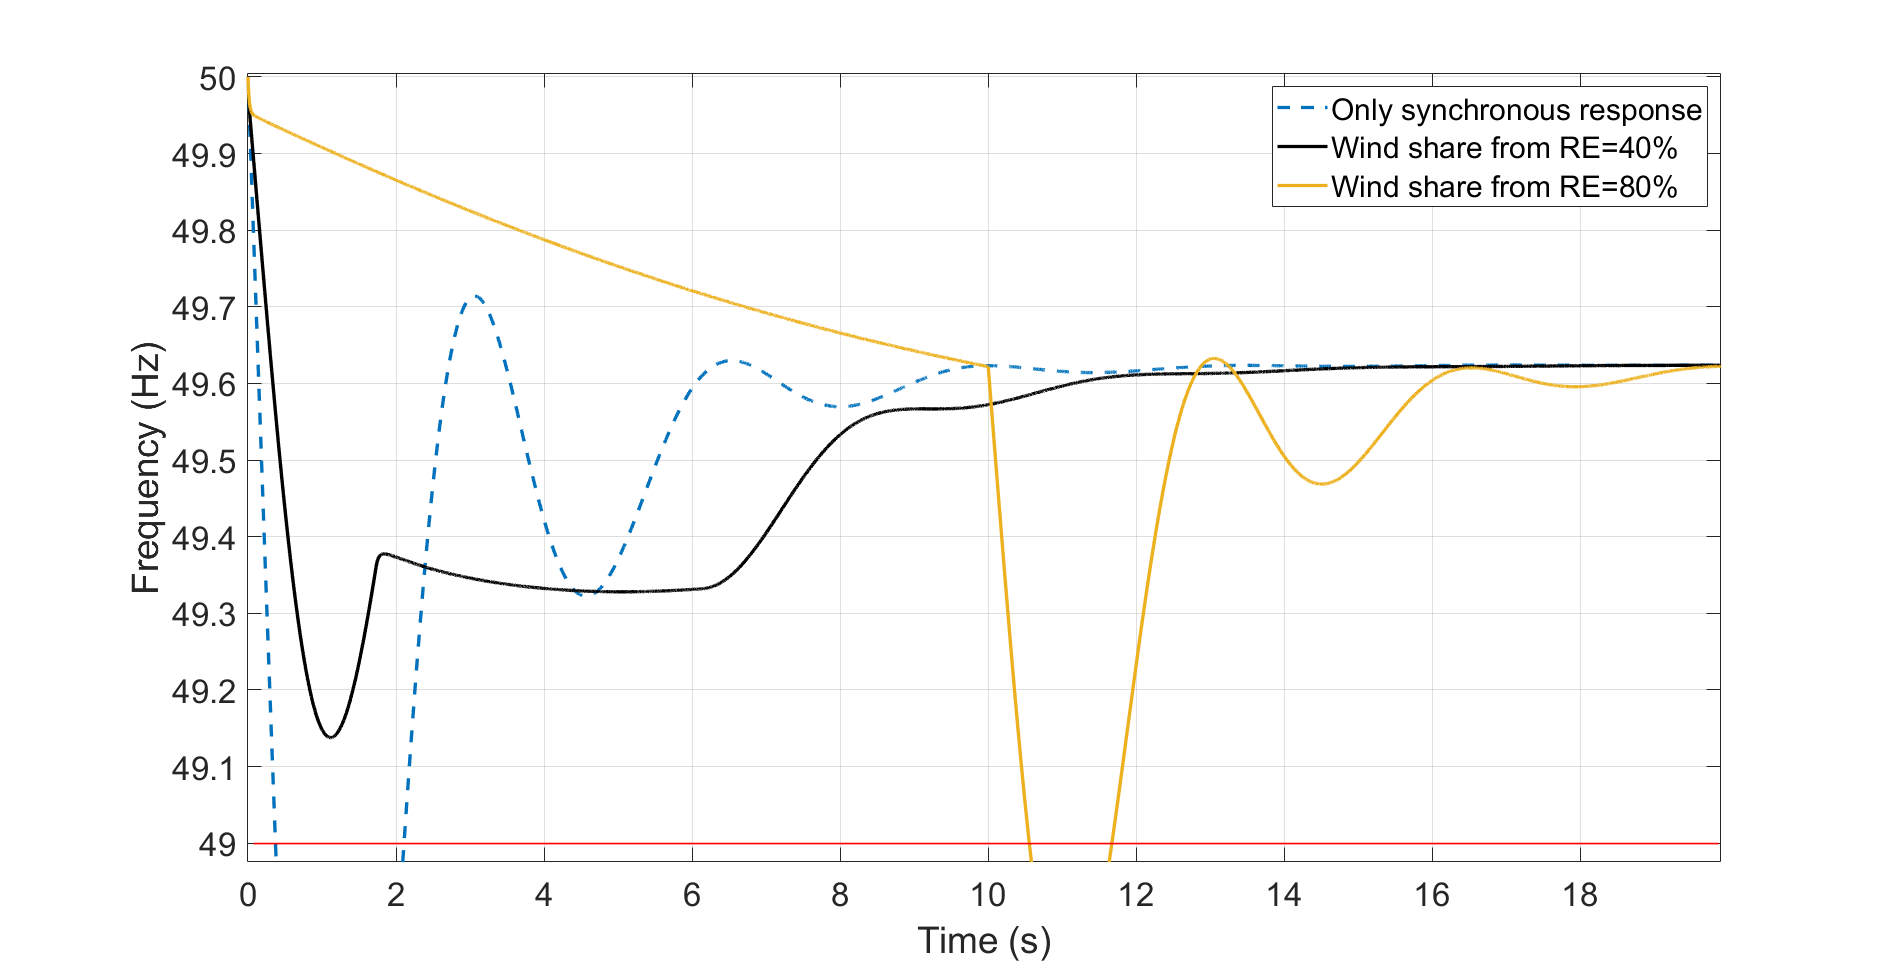
\includegraphics[width=\textwidth]{result/SI15imb}
		\caption{Simplified IEEE model with 15\% imbalance}
		\label{fig:res_ieee_fr15imb}
	\end{subfigure}
	\caption{Cases with contribution of 40\% and 80\% of the total IBG share are compared with the scenario with no support coming from IBG.}
\end{figure}


Figure \ref{fig:res_ieee_fr15imb} shows how a contribution of wind power of 40\% from the inverter-based generation is capable of avoiding UFLS. Nevertheless with the share of 80\% the frequency drops smoothly during a short period, then suddenly the frequency drops below 49 Hz. This situation leads to UFLS after 10 s because frequency has been sustained during that time by the synthetic inertia power. Since 10 seconds is the assumed time limit for exceeding the nominal turbine power rate; the synthetic inertia power, which has a big contribution to counteract the power imbalance, is switched off. On the other hand, when a higher imbalance occurs and the synthetic inertia response is saturated, due to the limitation of 10\% of rated power, the mechanical power increases at 10 seconds, having a less severe impact the switching off of the inertial response.


\subsubsection{Effect of Power Ramp Response on Frequency}

The contribution from the ramping power in diminishing system RoCoF from the inception of the perturbation until the critical time was disregarded when Equation \eqref{eq:p_at_tcr} was calculated. Assuming an instant switch-on of the IBFPR at the critical time, the frequency nadir would be 49 Hz. How ever, a ramp power response was assumed instead. Therefore the frequency response of an unbalanced system commonly exhibits a frequency nadir higher than 49 Hz due to the contribution of the ramping period. In this sense, it can be inferred that the longer the ramping period, the higher the frequency nadir that will be obtained. On the other hand, with the faster activation of IBFPR, the ramp slope and the steady power output can be diminished compromising frequency nadir. 

\begin{figure}[h]
	\centering
	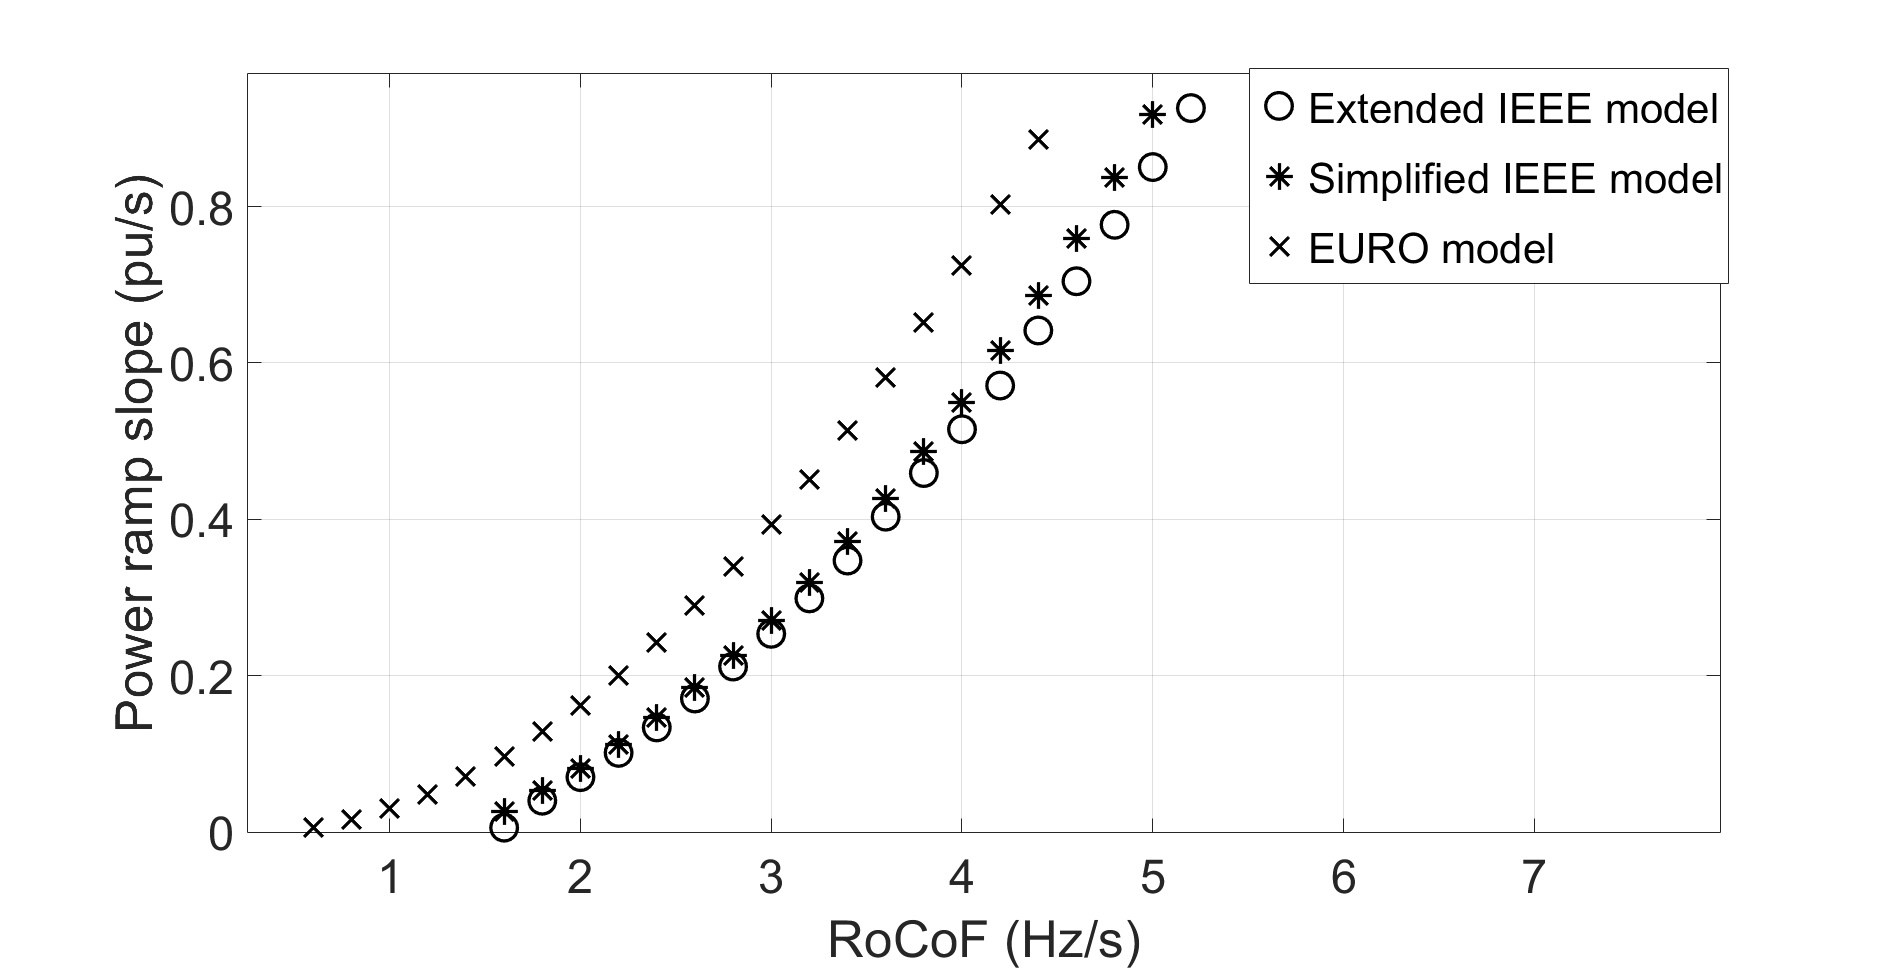
\includegraphics[width=0.6\textwidth]{/result/powerramps}
	\caption{Comparison of the results of the three models in terms of the IBFPR power ramp which is needed at 80\% of share from non-synchronous generation.}
	\label{fig:res_pramp}
\end{figure}

When a comparison is established between all the calculated power ramp slopes in per unit (pu), it can be noticed that with a high penetration of non-synchronous power in the system, the required power to ensure no UFLS have a consistent trend between the three models and proximity as seen in Figure \ref{fig:res_pramp}. A bigger amount of power ramp slope is needed in all the range of RoCoF for the European case. After inspecting Equation \ref{eq:IBFPR} it is noticed that the IBFPR is affected by the factor $ 1-t_{cr} /t_{nadir} $, then as nadir time increases, IBFPR increases as well. The nadir time for the European case, due to the action of the self-regulation and primary reserve deployment of 30 seconds, is in the range of 3-12 seconds (6 seconds for 80\% IBG penetration) whereas the nadir time for the simplified IEEE model is between 1-3 seconds.



\subsubsection{Fast Power Reserve}


The required power ramp to avoid load shedding has been found for both IEEE 9 bus models and the European-scale model. Hence, the IBFPR at the critical time, which remains constant after the critical time, would be accounted as the fast power reserve. In Table \ref{tb:crpowr} the required values for the inverter base reserve for the European model are listed for imbalances out of the reference case of ENTSOE.\\

\begin{table}[h]
	\caption{\label{tb:crpowr}: Fast power reserve in per unit for the European case. Power reserve expressed in pu with power load as the base}
	\centering
	%% \tablesize{} %% You can specify the fontsize here, e.g., \tablesize{\footnotesize}. If commented out \small will be used.
	\begin{tabular}{*9c}
		\toprule
		\textbf{IBG share (\%)}    & \multicolumn{8}{c}{\textbf{Load Imbalance (\%)}} \\
		\midrule
		{} & 3&    4&    5&    6&    7&    8&    9    &10 \\
		\midrule
		20&    -&    -&    0.025&    0.038&    0.049&    0.060&    0.070&    0.081\\
		40&    -&    0.016&    0.030&    0.041&    0.052&    0.063&    0.073&    0.083\\
		60&    0.005&    0.024&    0.035&    0.045&    0.056&    0.066&    0.077&    0.087\\
		80&    0.016&    0.028&    0.039&    0.049&    0.062&    0.070&    0.080&    0.09\\
		
		95&    0.024&    0.035&    0.045&    0.055&    0.065&    0.075&    0.085&    0.096\\
		\bottomrule
	\end{tabular}
\end{table}
\begin{figure}[h]
	\centering
	\begin{subfigure}[h]{0.49\textwidth}
		\centering
		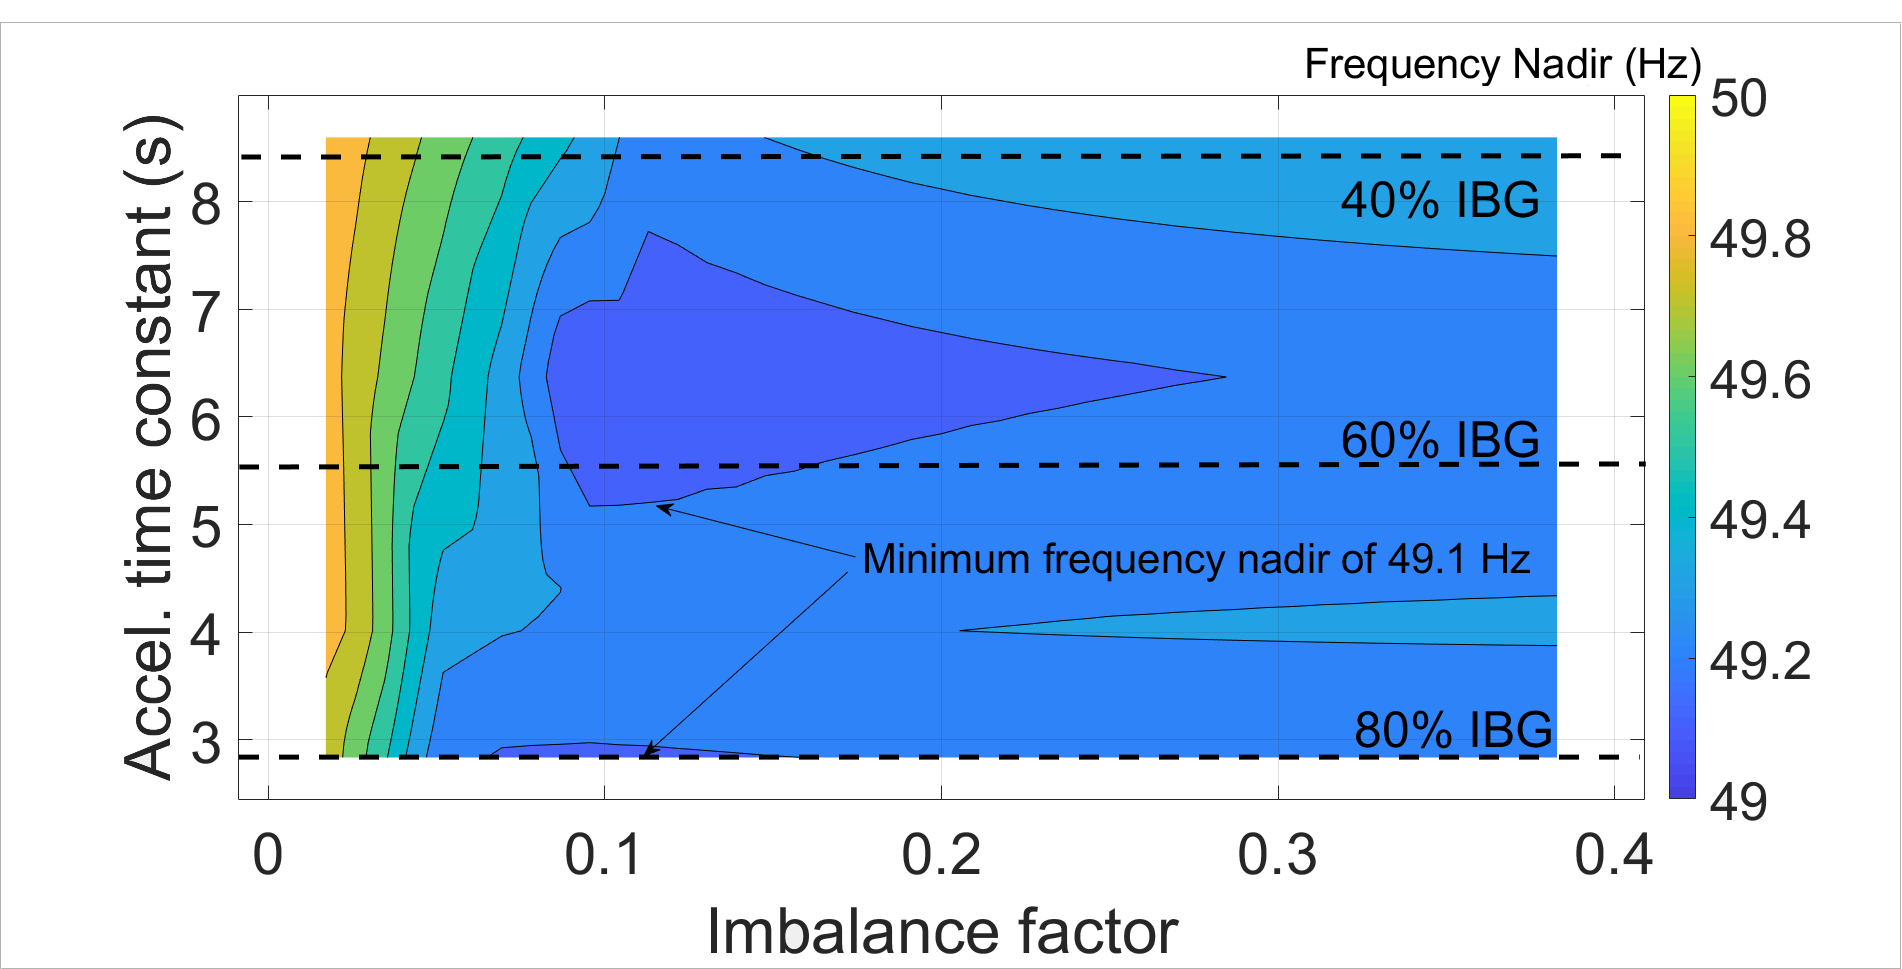
\includegraphics[width=\textwidth]{result/NadirIBFPR2}
		\caption{}
		\label{fig:res_ieee_ibfpr}
	\end{subfigure}
	\hfill
	\begin{subfigure}[h]{0.49\textwidth}
		\centering
		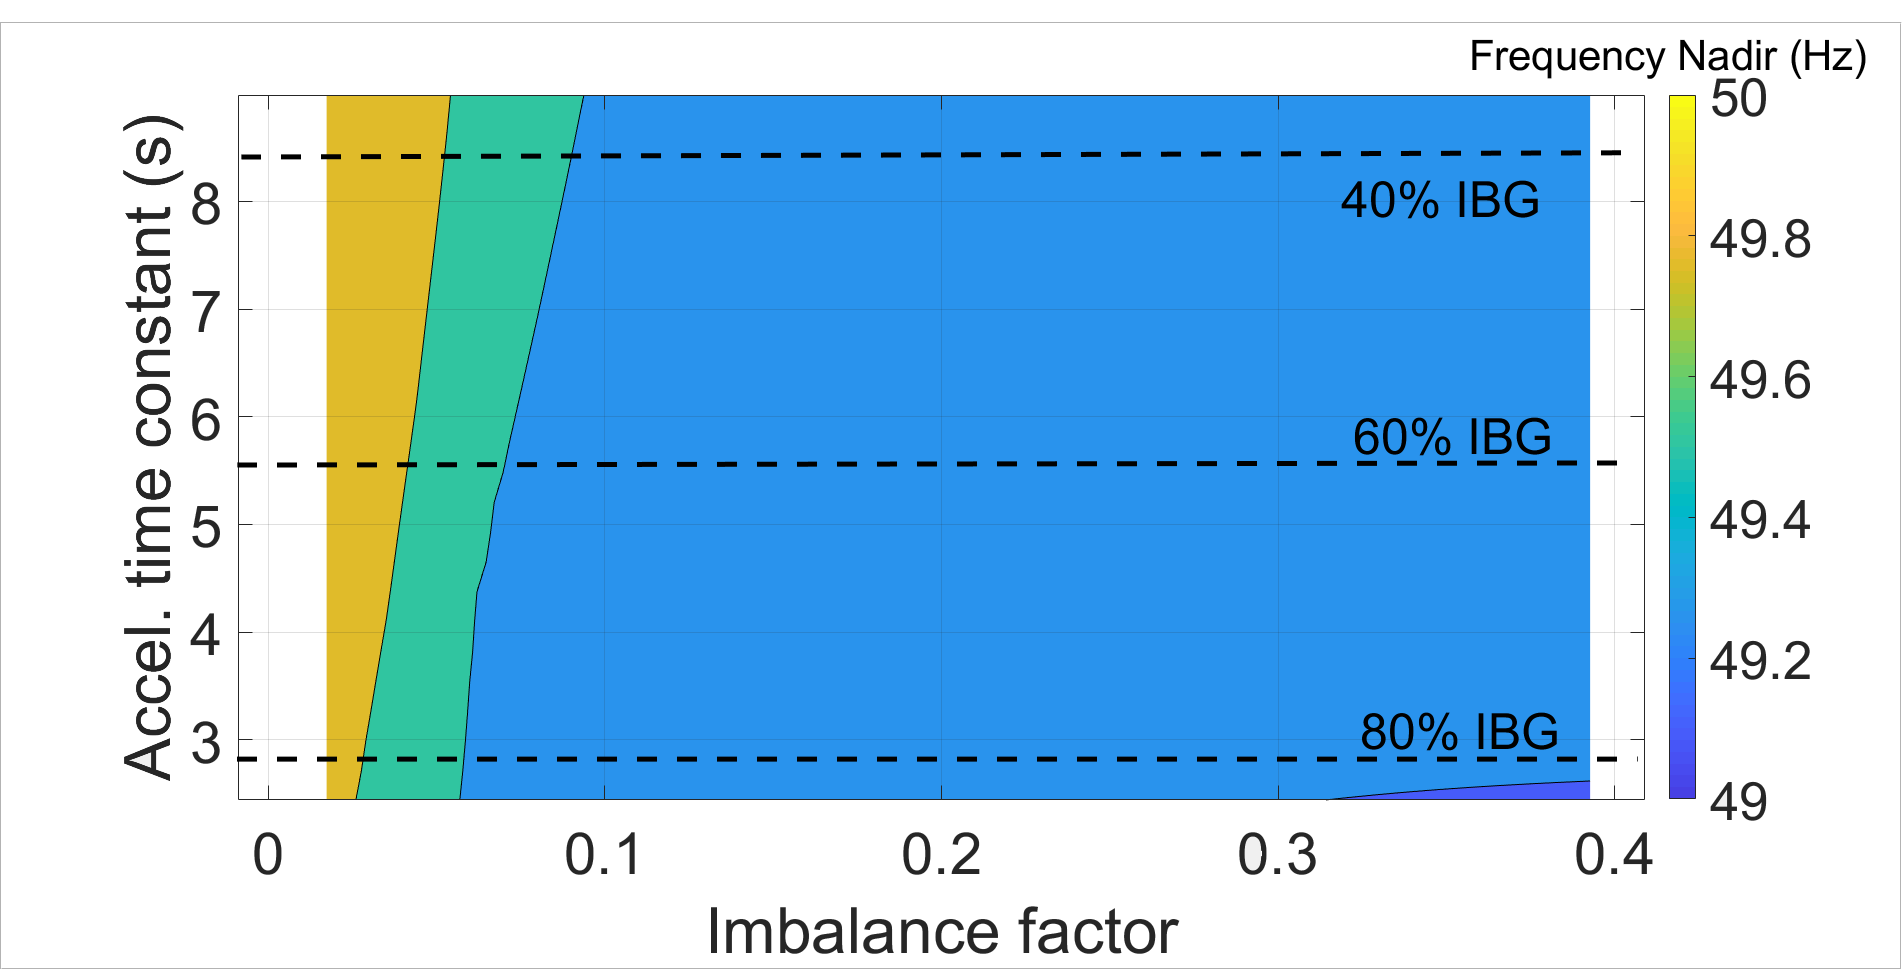
\includegraphics[width=\textwidth]{result/extnd}
		\caption{}
		\label{fig:res_extd_ibfpr}
	\end{subfigure}
	\hfill
	\begin{subfigure}[h]{0.48\textwidth}
		\centering
		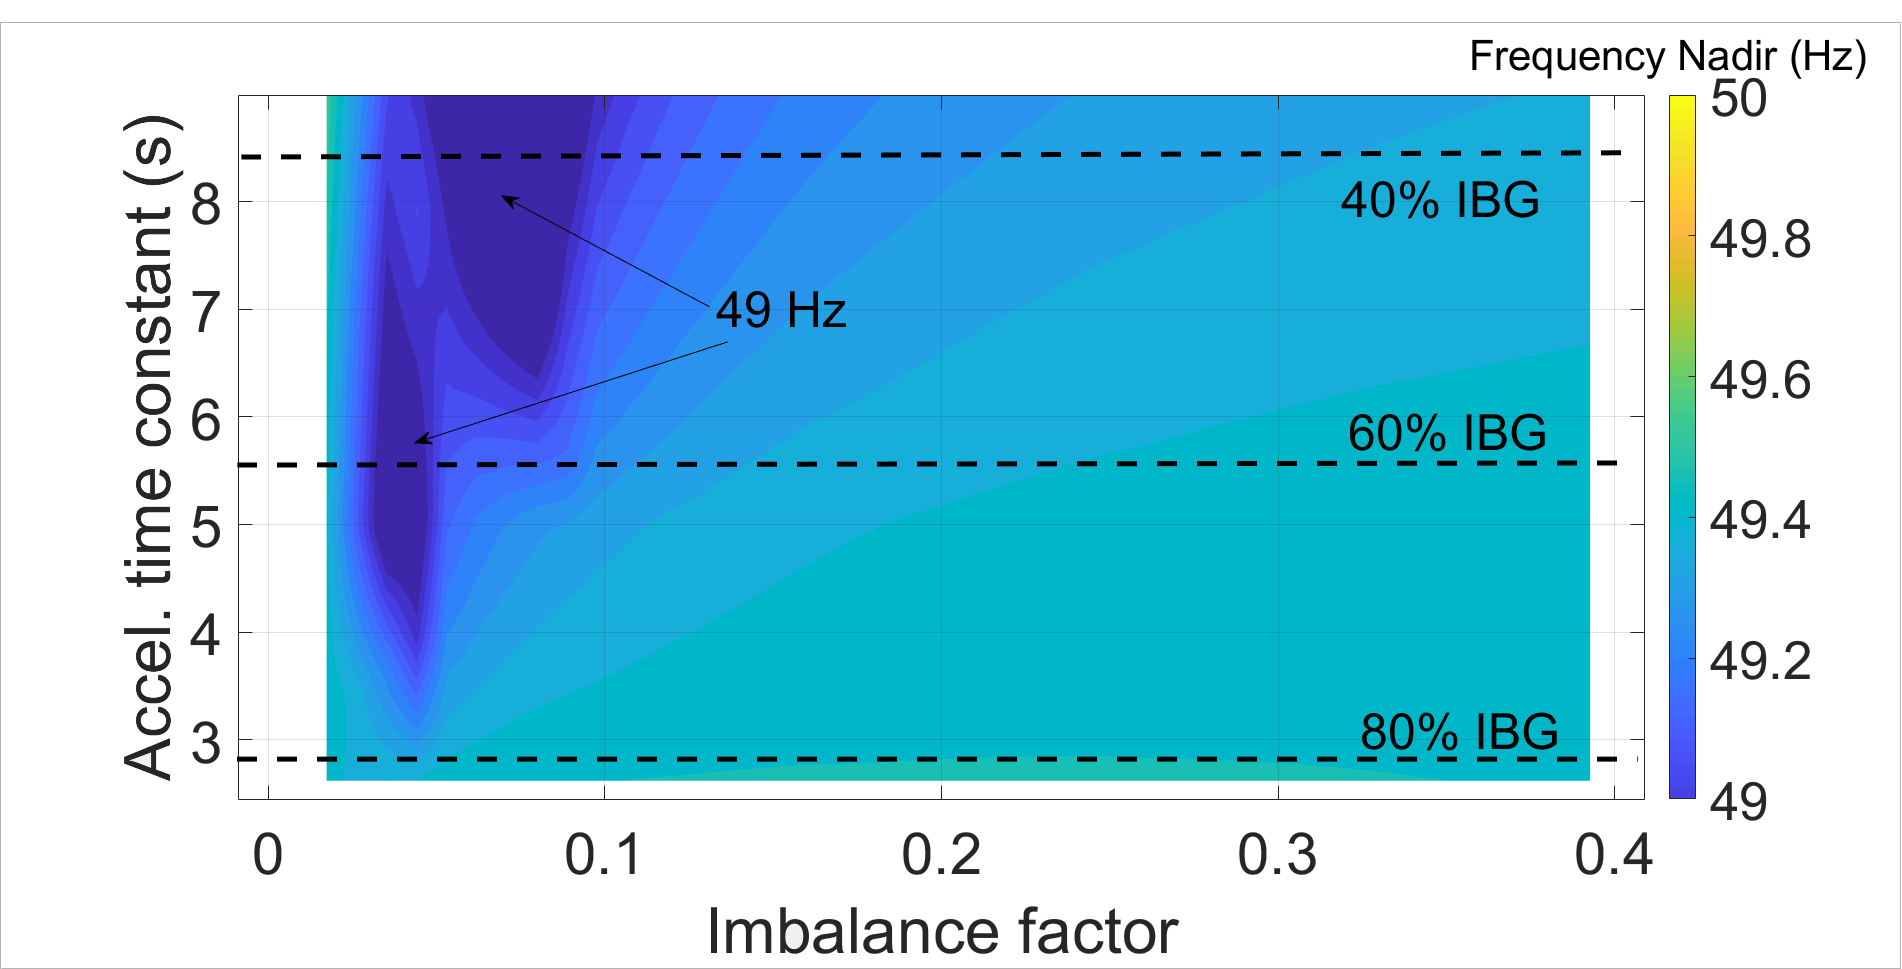
\includegraphics[width=\textwidth]{result/eu}
		\caption{}
		\label{fig:res_euro_ibfpr}
	\end{subfigure}
	
	
	\caption{Frequency nadir with the implementation of IBFPR in: (\textbf{a}) The simplified IEEE model  (\textbf{b}) The extended IEEE model. (\textbf{c}) The large scale (European model). }
\end{figure}
When IBFPR is implemented in all three cases, frequency drop below 49 Hz is avoided for almost all values of RoCoF, provided that enough IBFPR is available for the given imbalance. Figures \ref{fig:res_ieee_ibfpr} to \ref{fig:res_euro_ibfpr} show the frequency nadir for all the cases.\\


It can be observed that in the IEEE grid models, depicted in Figure \ref{fig:res_ieee_ibfpr} and \ref{fig:res_extd_ibfpr}, that UFLS is avoided in all the cases. However, in the simplified IEEE model, a minima area with a value of 49.1 Hz is found as indicated in the figure. This is caused due to the selected values of time constants for such inertia scenario. As indicated in Table \ref{tb:timeconstant} the generator with a capacity of 590 MVA has a bigger reheat time constant than the other machines, causing a delay in synchronous response. As the imbalance increases, the relevance of such response diminishes, therefore frequency nadir increases. In the case of the extended IEEE model, time constants were kept equal for all inertia scenarios and only generator inertia was changed. In the European-scale model depicted in Figure \ref{fig:res_euro_ibfpr}, UFLS is not avoided in the region of low imbalance and high acceleration time constant. Since the implemented IBFPR was based on a power response as a function of the measured RoCoF, the inaccuracy in the fit function leads to overestimating the critical time in the low region of RoCoF. This has a bigger influence on the European-scale model because such inaccuracy is not compensated by a faster power response from the synchronous machines.

\begin{figure}[h]
	\centering
	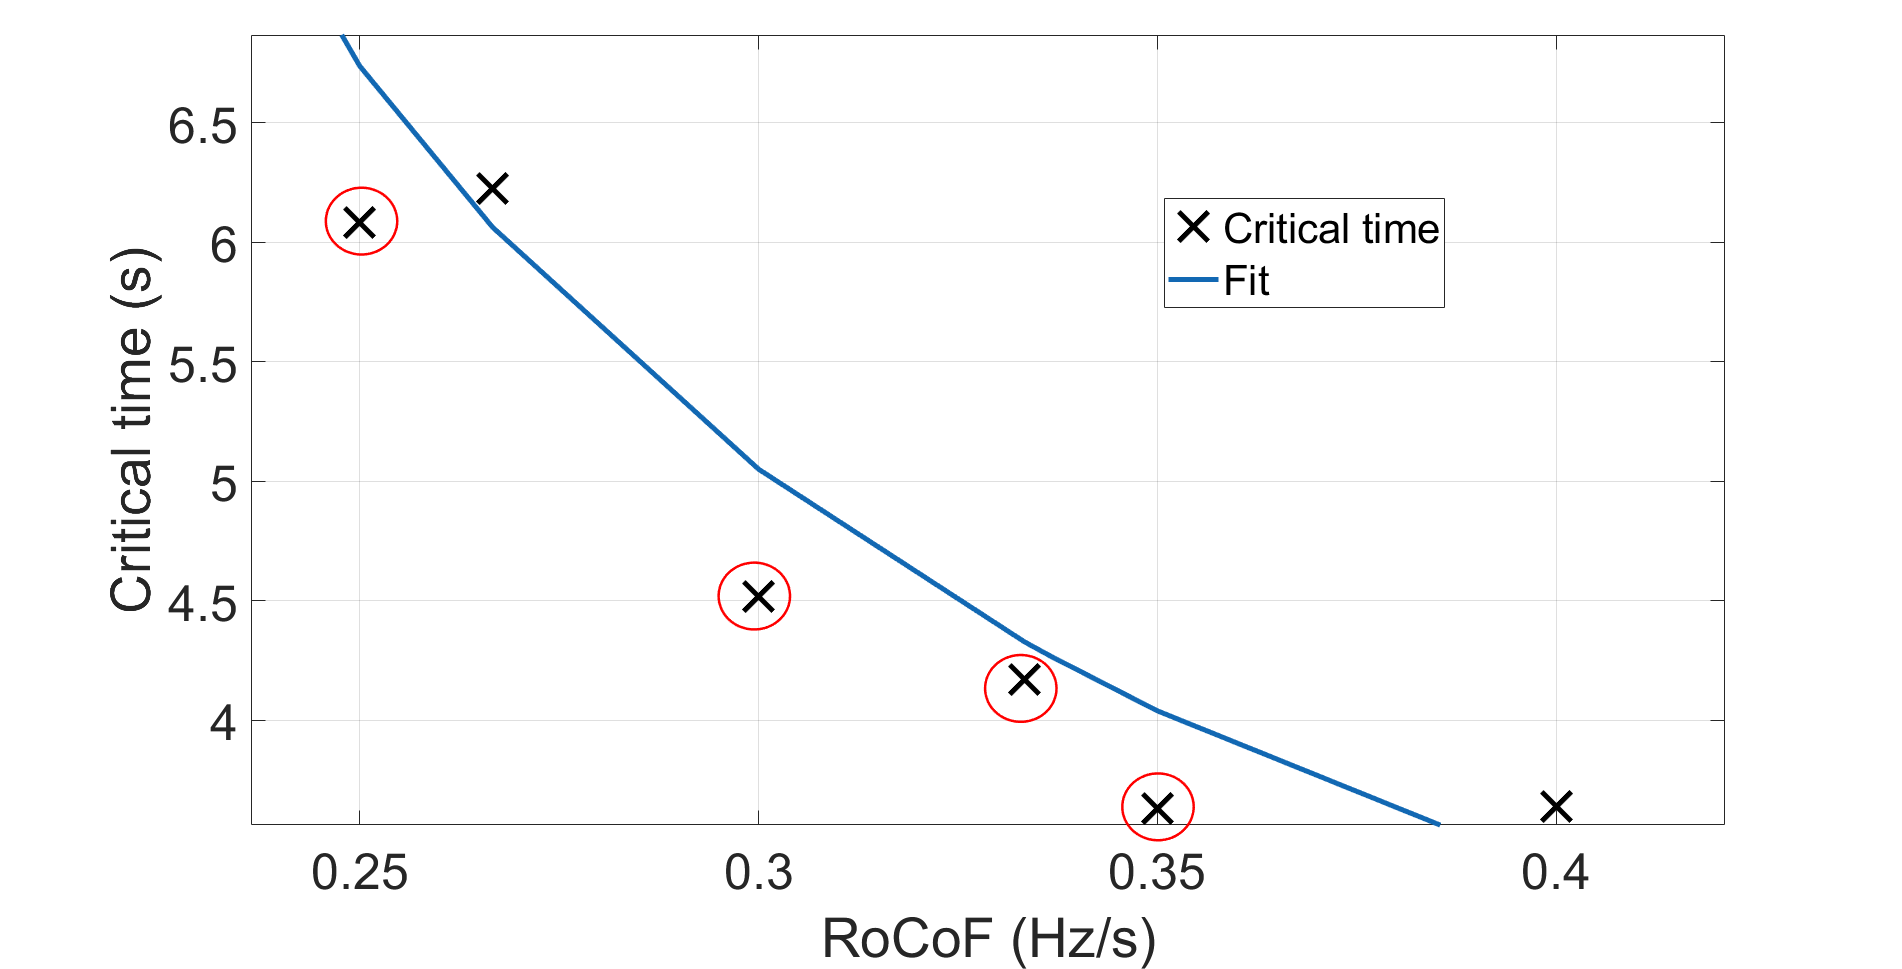
\includegraphics[width=0.5\textwidth]{/result/fit}
	\caption{Overestimation of critical time leading to UFLS in the European-scale model.}
	\label{fig:res_fit}
\end{figure}

\subsection{Synchronizing effect, lack of damping torque and implications}

The diminishing of synchronous machines in the system leads to a very weak network where synchronizing and damping torque, which are inherent characteristics of synchronous machines, are not enough to stabilize the system \cite{kundur1994power}. Although the implementation of IBFPR contributes to keeping the synchronous machine on step, oscillations in the speed/frequency response of the rotor are observed. These oscillations are created by the lack of damping torque which is provided mainly by the synchronous machines through damping windings, rotor field exciter, and power system stabilizer \cite{kundur1994power}. 

\begin{figure}[h]
	\centering
	\begin{subfigure}[h]{0.49\textwidth}
		\centering
		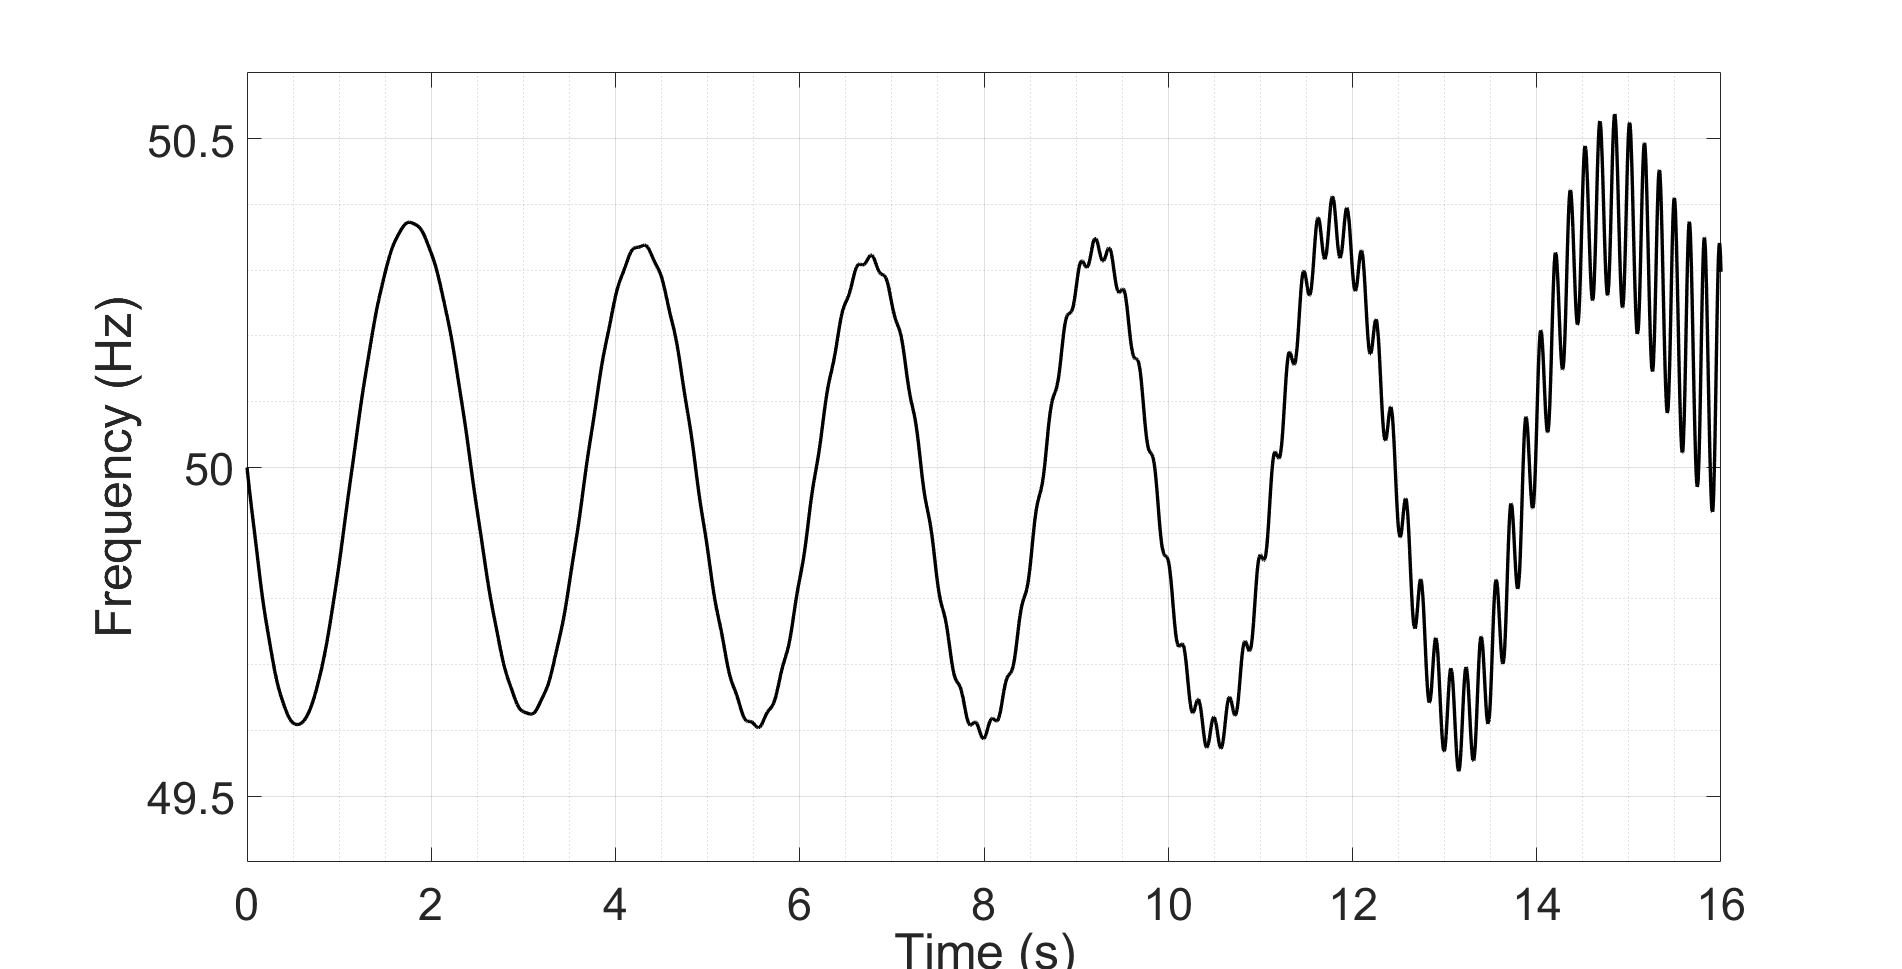
\includegraphics[width=\textwidth]{result/Smallsignal}
		\caption{Without IBFPR}
		\label{fig:res_osc_noIBFPR}
	\end{subfigure}
	\hfill
	\begin{subfigure}[h]{0.49\textwidth}
		\centering
		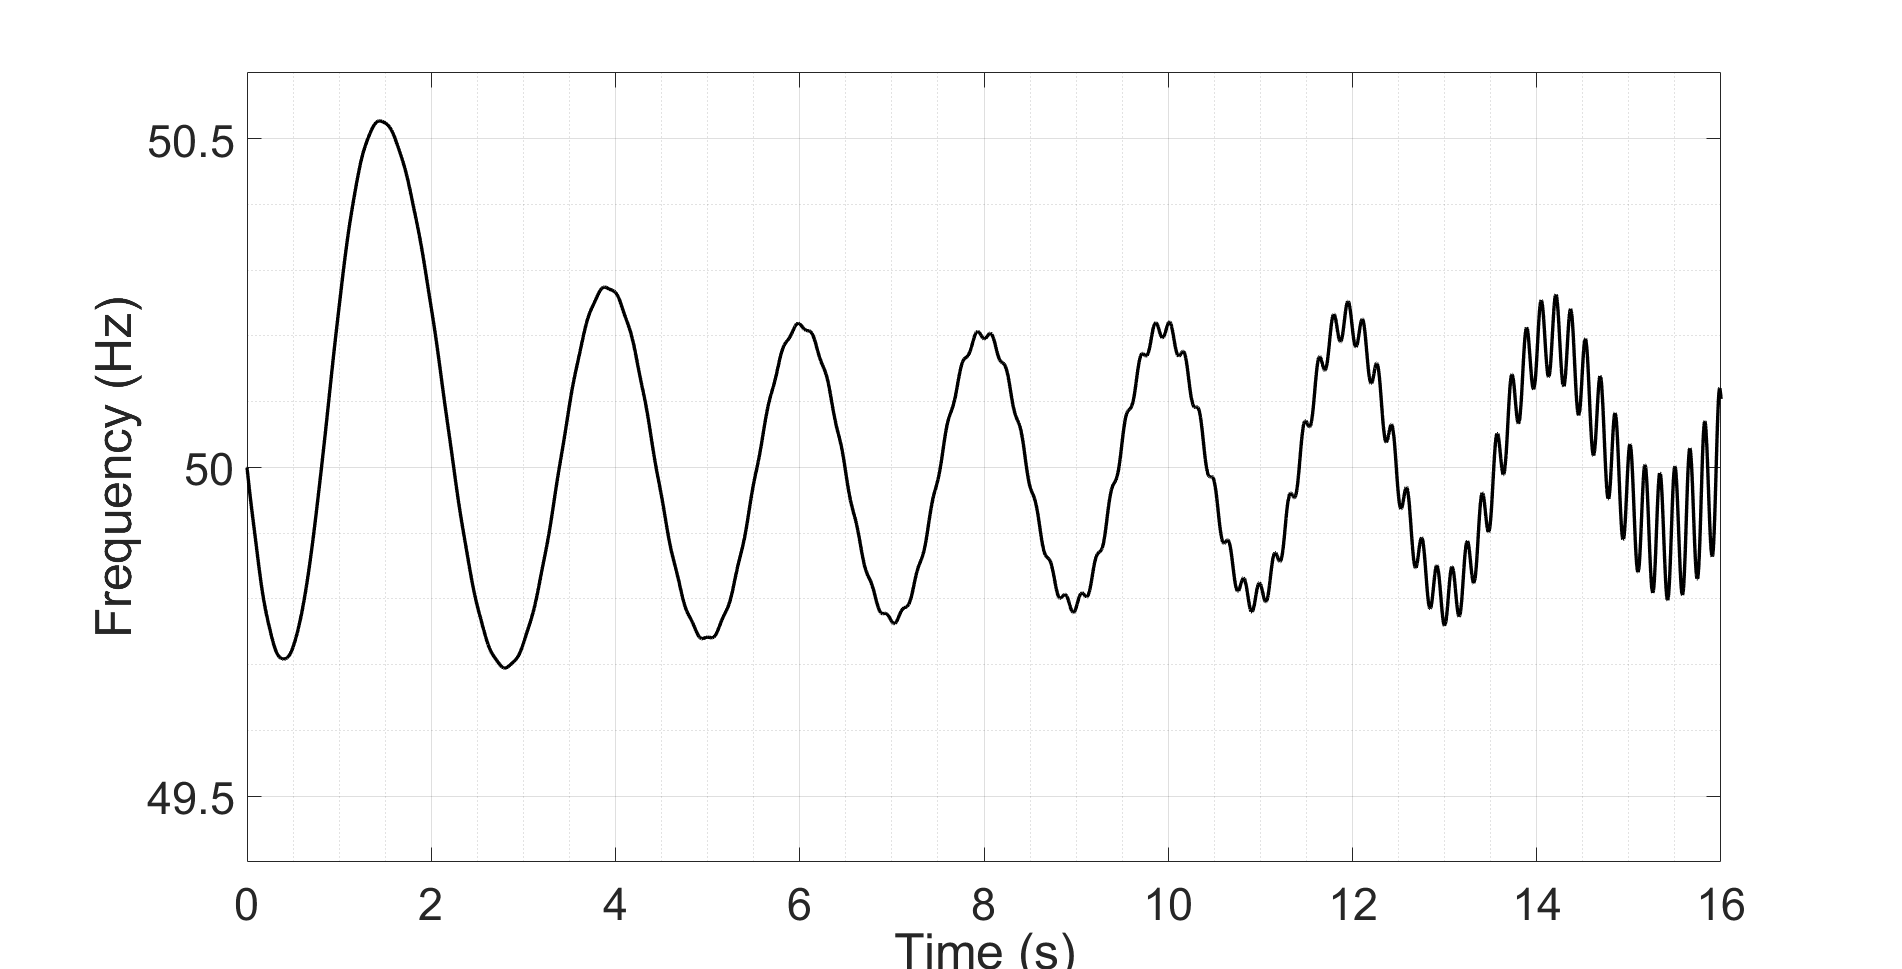
\includegraphics[width=\textwidth]{result/Smallsignal2}
		\caption{With IBFPR}
		\label{fig:res_osc_IBFPR}
	\end{subfigure}
	
	
	\caption{In (\textbf{a}) the oscillatory frequency response is depicted when no additional frequency support is given by the IBG, whereas in  (\textbf{b}) the IBFPR is applied. In both cases an imbalance of 2\% and a penetration of 95\% of IBG were considered.}
\end{figure}


For the simplified IEEE model and the European-scale model, only transfer functions describing an equivalent system governor were considered. Hence in such approaches, the effect and dynamics of synchronous generator’s exciters and inter-machine interaction were not taken into account. The before mention factors influence greatly small signal stability \cite{kundur1994power, Anderson.2002}. Even though the scope of this work was to analyze the power-time characteristics needed to avoid frequency collapse; oscillations were observed but they could not be addressed by the simple injection of power to the system. When penetration of 95\% of inverter-based generation and 2\% of load imbalance is considered, UFLS is not reached but the system becomes unstable as shown in Figure \ref{fig:res_osc_noIBFPR} and Figure \ref{fig:res_osc_IBFPR}. With penetrations levels above 85\%, complete frequency stability is not ensured with the injection of fast power reserve. Then the system becomes unstable with increasing amplitude oscillations. It is important to note that ENTSOE in its EUROPEAN interconnected scenario determined that there is no UFLS when an imbalance of 2\% with a high contribution of non-synchronous generation occurs.  Nonetheless, no inter-machine interaction was considered and therefore a similar effect as the one in \ref{fig:res_osc_noIBFPR} could be experienced.